\documentclass{article}
\usepackage[utf8]{inputenc}
\usepackage[T1]{fontenc}
\usepackage[french]{babel}
\usepackage{amsmath,amsfonts,amssymb,amsthm}
\usepackage[margin=2.5cm]{geometry}
\usepackage{graphicx}

\begin{document}

\paragraph{Introduction}
En ce qui concerne les diagrammes de séquence de l'application pour les institutions.
Nous avons fait le choix pour un bon nombre d'entre eux de ne pas les réaliser pour l'une
de deux raisons
\begin{enumerate}
    \item Le diagramme est considéré comme trivial comme expliqué dans la partie client
    \item Le diagramme a un équivalent dans la partie client et serait donc redondant
\end{enumerate}

Nous avons donc réalisé les diagrammes de séquence des interactions les plus complexes.

\paragraph{Accéder à la liste des demandes}
Cette interaction permet à la banque d'accéder à la liste des demandes que ses utilisateurs
ont postés. Elle démarre à la création de la scène RequestScene (1) qui va réaliser un appel
à l'API avec getNotification en précisant le numéro SWIFT de la banque dont l'on veut récupérer
les notifications(2). Le serveur répondra avec une liste de notifications(3). Une fois que
l'application a reçu les données, elle affichera la liste avec la méthode display(4).

\begin{figure}[h!]
    \hbox{
        \centering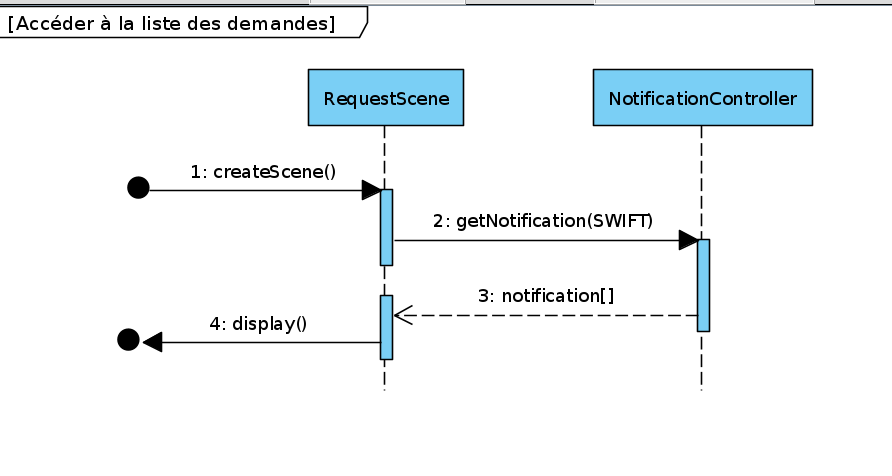
\includegraphics[width=\linewidth]{../img/sequence-institution-img1.png}% modif img path
    }
    \caption{Accéder à la liste des demandes}
\end{figure}

\newpage

\paragraph{Approuver une demande}
Lorsqu'un objet Request recoit une demande d'approbation(1), il enverra à l'API une demande pour créer
une notification afin d'informer l'utilisateur qui a introduit la requête que sa demande a été acceptée(2).
Ensuite elle enverra une 2e demande à l'API pour cette fois si delete cette request du serveur(3).

\begin{figure}[h!]
    \hbox{
        \centering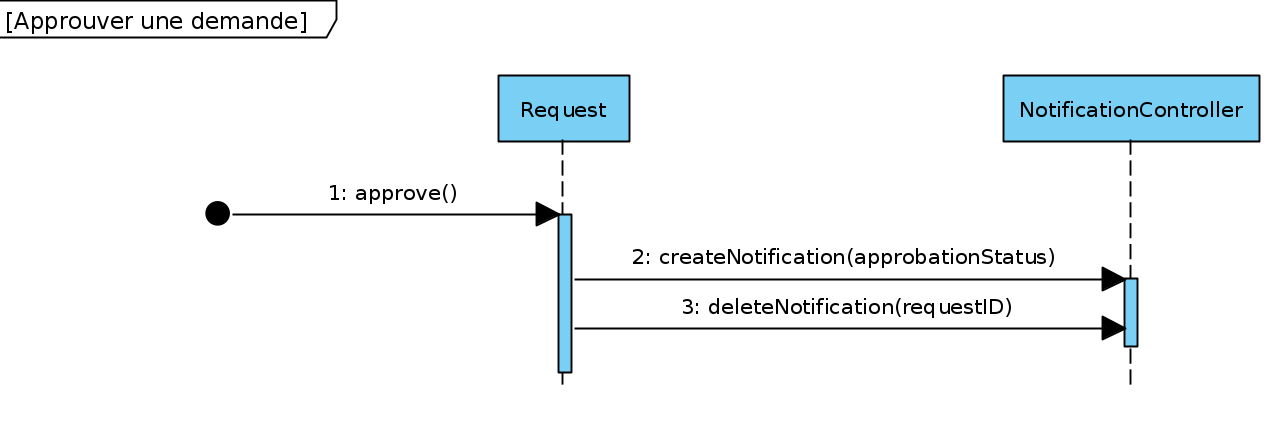
\includegraphics[width=\linewidth]{../img/sequence-institution-img2.png}% modif img path
    }
    \caption{Approuver une demande}
\end{figure}

\newpage

\paragraph{Ouvrir un produit financier}
L'interaction commence quand la banque entre les donnnés du produit financier qui sont: clientName,
clientID, IBAN, accountType (1). Lorsqu'il actionnera le bouton pour créer le produit, la scène fera
un appel à l'API pour créer le produit(2). Si les données reçues par le WalletController sont correctes,
Une notification sera créer pour informer le client que son produit a été ouvert(4). Ensuite la scène
informera la banque que la requête a été effectuée avec succès(5). Si les données reçues par le
WalletController sont incorrectes, l'application affichera un message d'erreur(6). 

\begin{figure}[h!]
    \hbox{
        \centering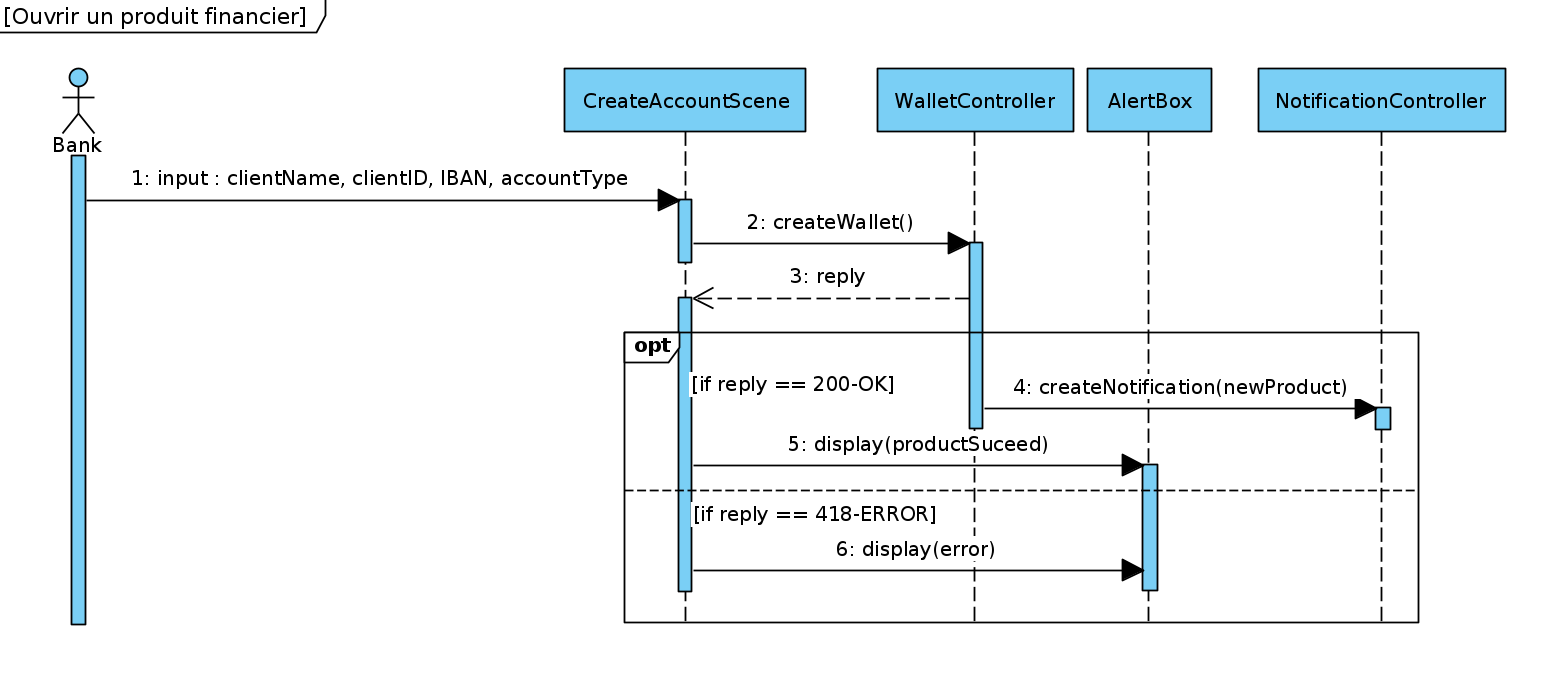
\includegraphics[width=\linewidth]{../img/sequence-institution-img3.png}% modif img path
    }
    \caption{Ouvrir un produit financier}
\end{figure}

\end{document}